\documentclass[xcolor=table,dvipsnames,table]{beamer}
\mode<presentation>
\usetheme{boxes}
\setbeamertemplate{navigation symbols}{}
% http://www.latex-community.org/forum/viewtopic.php?f=4&t=6694
\setbeamertemplate{navigation symbols}{\raisebox{5pt}{\makebox[\paperwidth]{\hfill\makebox[10pt]{\scriptsize\insertframenumber\vspace{1ex}}}}}
%\setbeamertemplate{footline}[frame number]
\setbeamertemplate{blocks}[shadow=false]
%\setbeamercolor*{block title}{fg=structure,bg=RoyalBlue!10}
\setbeamercolor*{block title example}{fg=structure,bg=RoyalBlue!10}
%\setbeamercolor*{block title example}{fg=BrickRed,bg=Goldenrod!10}
\setbeamercolor*{block title alerted}{fg=white,bg=black}
\addtobeamertemplate{block begin}{\pgfsetfillopacity{0.8}}{\pgfsetfillopacity{1}}
%\rowcolors{0}{RoyalBlue!20}{RoyalBlue!5}

%\DeclareGraphicsRule{*}{mps}{*}{}

\usepackage{latexsym}
\usepackage{hyperref}
\usepackage{tikz}
\usetikzlibrary{calc,shapes,arrows,shadows,shapes.callouts,shapes.arrows,chains,positioning,trees}
\usepackage{solution}
\usepackage{calc}
\usepackage{pifont}
\usepackage{algorithmic}

\newcommand{\cmark}{\ding{51}}
\newcommand{\xmark}{\ding{55}}

\newcounter{mycallout}

\newcommand{\callouts}[3]{%
  \stepcounter{mycallout}
  \tikz[remember picture,baseline]{\node[anchor=base,inner sep=0,outer sep=0]%
    (\themycallout) {\colorbox{#1!20}{#3}};\pause\node[overlay,rectangle callout,%
    callout relative pointer={(0cm,0.5cm)},fill=#1!20] at ($(\themycallout.south)+(-0cm,-0.7cm)$){#2};}%
    }%

\raggedright

\newcount\lecturecount
\lecturecount=0
\AtBeginLecture{%
    \advance\lecturecount by 1
    \date{}
    \begin{frame}
    \begin{center}
    \titlepage
    \ifnum\lecturecount=1
    Part \the\lecturecount: \insertlecture
    \else
    Part \the\lecturecount: \insertlecture
    \fi
    \end{center}
    \end{frame}
}

\addtobeamertemplate{block begin}{\setlength\abovedisplayskip{0pt}}

%\newcommand{\example}[1]{{\color{BrickRed!50}{#1}}}
\newcommand{\maths}[1]{{\color{RoyalBlue!50}{#1}}}
\newcommand{\reference}[1]{{\color{RoyalBlue!30}\tiny [from #1]}}
\newcommand{\koehnref}{\reference{\href{http://www.statmt.org/book}{P.Koehn SMT book slides}}}


\begin{document}

\title{\color{RoyalBlue!20}Natural Language Processing}

\author{Anoop Sarkar \\ {\tt anoopsarkar.github.io/nlp-class}}
\institute{Simon Fraser University}
%\date{}
     
{
\setbeamertemplate{navigation symbols}{}
\addtocounter{framenumber}{-1}
\begin{frame}
\begin{center}
\vspace{8mm}
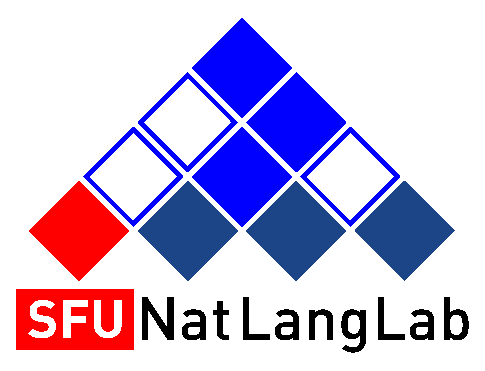
\includegraphics[scale=0.35]{figures/natlang-cky-logo}
\end{center}
\titlepage
\end{frame}
}



\lecture{Neural Language Models}{}
\section{Log-linear Language Models}

\begin{frame}
\frametitle{The Language Modeling problem}
\begin{block}{Setup}
\begin{itemize}[<+->]
\item Assume a (finite) vocabulary of words:
\[ {\cal V} = \{ killer, crazy, clown \} \]
\item Use ${\cal V}$ to construct an infinite set of \textit{sentences} 
\begin{eqnarray*} 
{\cal V}^+ = & \{ & \\
&& \mbox{clown, killer clown, crazy clown, } \\
&& \mbox{crazy killer clown, killer crazy clown}, \\
&& \ldots \\
& \} &
\end{eqnarray*}
\item A \textit{sentence} is \textbf{defined} as each $s \in {\cal V}^+$
\end{itemize}
\end{block}
\end{frame}


\section*{Acknowledgements}

\begin{frame}
\centering
\begin{alertblock}{Acknowledgements}
Many slides borrowed or inspired from lecture notes by Michael Collins, Chris Dyer, Kevin Knight, Chris Manning, Philipp Koehn, Adam Lopez, Graham Neubig, Richard Socher and Luke Zettlemoyer from their NLP course materials. 

\bigskip

All mistakes are my own.

\bigskip

A big thank you to all the students who read through these notes and helped me improve them.

\end{alertblock}
\end{frame}



\end{document}
